% Figure 1.1: Timeline of Number Systems
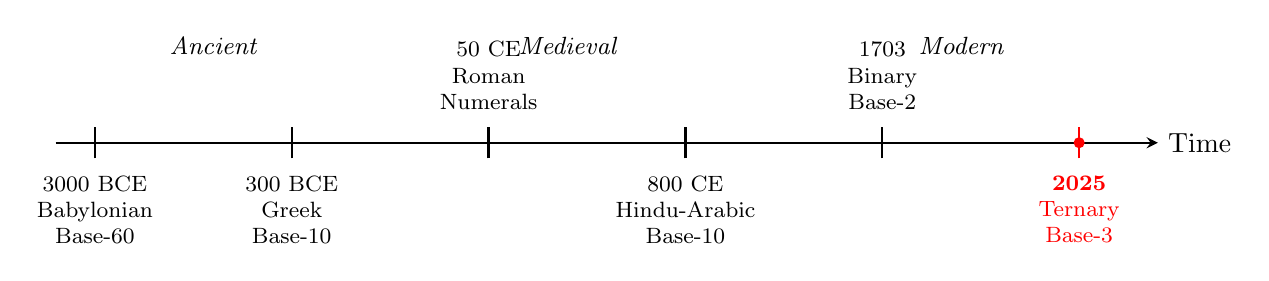
\begin{tikzpicture}[scale=1.0]
  % Timeline axis
  \draw[thick, ->, >=stealth] (0,0) -- (14,0) node[right] {Time};

  % Historical markers
  \def\timelinedata{
    {0.5, "3000 BCE", "Babylonian", "Base-60"},
    {3.0, "300 BCE", "Greek", "Base-10"},
    {5.5, "50 CE", "Roman", "Numerals"},
    {8.0, "800 CE", "Hindu-Arabic", "Base-10"},
    {10.5, "1703", "Binary", "Base-2 (Leibniz)"},
    {13.0, "2025", "Ternary", "Base-3 (This Book)"}
  }

  % Babylonian (3000 BCE)
  \draw[thick] (0.5,-0.2) -- (0.5,0.2);
  \node[below, align=center, font=\footnotesize] at (0.5,-0.3) {3000 BCE\\Babylonian\\Base-60};

  % Greek (300 BCE)
  \draw[thick] (3.0,-0.2) -- (3.0,0.2);
  \node[below, align=center, font=\footnotesize] at (3.0,-0.3) {300 BCE\\Greek\\Base-10};

  % Roman (50 CE)
  \draw[thick] (5.5,-0.2) -- (5.5,0.2);
  \node[above, align=center, font=\footnotesize] at (5.5,0.3) {50 CE\\Roman\\Numerals};

  % Hindu-Arabic (800 CE)
  \draw[thick] (8.0,-0.2) -- (8.0,0.2);
  \node[below, align=center, font=\footnotesize] at (8.0,-0.3) {800 CE\\Hindu-Arabic\\Base-10};

  % Binary (1703)
  \draw[thick] (10.5,-0.2) -- (10.5,0.2);
  \node[above, align=center, font=\footnotesize] at (10.5,0.3) {1703\\Binary\\Base-2};

  % Ternary (2025) - highlighted
  \draw[thick, red] (13.0,-0.2) -- (13.0,0.2);
  \node[below, align=center, font=\footnotesize, red] at (13.0,-0.3) {\textbf{2025}\\Ternary\\Base-3};
  \fill[red] (13.0,0) circle (2pt);

  % Era labels
  \node[above, font=\small\itshape] at (2.0,1.0) {Ancient};
  \node[above, font=\small\itshape] at (6.5,1.0) {Medieval};
  \node[above, font=\small\itshape] at (11.5,1.0) {Modern};

\end{tikzpicture}
